\documentclass[12pt,a4paper]{article}
\usepackage{amsmath,amssymb,mathrsfs,tikz,times,pifont}
\usepackage{enumitem}
\newcommand\circitem[1]{%
\tikz[baseline=(char.base)]{
\node[circle,draw=gray, fill=red!55,
minimum size=1.2em,inner sep=0] (char) {#1};}}
\newcommand\boxitem[1]{%
\tikz[baseline=(char.base)]{
\node[fill=cyan,
minimum size=1.2em,inner sep=0] (char) {#1};}}
\setlist[enumerate,1]{label=\protect\circitem{\arabic*}}
\setlist[enumerate,2]{label=\protect\boxitem{\alph*}}
%%%::::::by chnini ameur :::::::%%%
\everymath{\displaystyle}
\usepackage[left=1cm,right=1cm,top=1cm,bottom=1.7cm]{geometry}
\usepackage[colorlinks=true, linkcolor=blue, urlcolor=blue, citecolor=blue]{hyperref}
\usepackage{array,multirow}
\usepackage[most]{tcolorbox}
\usepackage{varwidth}
\usepackage{float} %pour utiliser l'option [H] qui force l'image à apparaître exactement à l'endroit où elle est placée dans le code.
\tcbuselibrary{skins,hooks}
\usetikzlibrary{patterns}
%%%::::::by chnini ameur :::::::%%%
\newtcolorbox{exa}[2][]{enhanced,breakable,before skip=2mm,after skip=5mm,
colback=yellow!20!white,colframe=black!20!blue,boxrule=0.5mm,
attach boxed title to top left ={xshift=0.6cm,yshift*=1mm-\tcboxedtitleheight},
fonttitle=\bfseries,
title={#2},#1,
% varwidth boxed title*=-3cm,
boxed title style={frame code={
\path[fill=tcbcolback!30!black]
([yshift=-1mm,xshift=-1mm]frame.north west)
arc[start angle=0,end angle=180,radius=1mm]
([yshift=-1mm,xshift=1mm]frame.north east)
arc[start angle=180,end angle=0,radius=1mm];
\path[left color=tcbcolback!60!black,right color = tcbcolback!60!black,
middle color = tcbcolback!80!black]
([xshift=-2mm]frame.north west) -- ([xshift=2mm]frame.north east)
[rounded corners=1mm]-- ([xshift=1mm,yshift=-1mm]frame.north east)
-- (frame.south east) -- (frame.south west)
-- ([xshift=-1mm,yshift=-1mm]frame.north west)
[sharp corners]-- cycle;
},interior engine=empty,
},interior style={top color=yellow!5}}
%%%%%%%%%%%%%%%%%%%%%%%

\usepackage{fancyhdr}
\usepackage{eso-pic}         % Pour ajouter des éléments en arrière-plan
% Commande pour ajouter du texte en arrière-plan
\usepackage{tkz-tab}
\AddToShipoutPicture{
    \AtTextCenter{%
        \makebox[0pt]{\rotatebox{80}{\textcolor[gray]{0.7}{\fontsize{5cm}{5cm}\selectfont PGB}}}
    }
}
\usepackage{lastpage}
\fancyhf{}
\pagestyle{fancy}
\renewcommand{\footrulewidth}{1pt}
\renewcommand{\headrulewidth}{0pt}
\renewcommand{\footruleskip}{10pt}
\fancyfoot[R]{
\color{blue}\ding{45}\ \textbf{2024}
}
\fancyfoot[L]{
\color{blue}\ding{45}\ \textbf{Prof:M. BA}
}
\cfoot{\bf
\thepage /
\pageref{LastPage}}

% Définition de l'encadré adaptatif avec fond jaune
\newtcolorbox{resultbox}{
    colback=red!30, % Fond rouge clair
    colframe=black, % Bordure noire fine
    sharp corners, % Coins nets
    boxrule=0.5pt, % Contour léger
    boxsep=2pt, % Espacement interne
    left=5pt, right=5pt, top=2pt, bottom=2pt, % Marges internes
}

\begin{document}
\renewcommand{\arraystretch}{1.5}
\renewcommand{\arrayrulewidth}{1.2pt}
\begin{tikzpicture}[overlay,remember picture]
\node[draw=blue,line width=1.2pt,fill=purple,text=blue,inner sep=3mm,rounded corners,pattern=dots]at ([yshift=-2.5cm]current page.north) {\begingroup\setlength{\fboxsep}{0pt}\colorbox{white}{\begin{tabular}{|*1{>{\centering \arraybackslash}p{0.28\textwidth}} |*2{>{\centering \arraybackslash}p{0.2\textwidth}|} *1{>{\centering \arraybackslash}p{0.19\textwidth}|} }
\hline
\multicolumn{3}{|c|}{$\diamond$$\diamond$$\diamond$\ \textbf{Lycée de Dindéfélo}\ $\diamond$$\diamond$$\diamond$ }& \textbf{A.S. : 2024/2025} \\ \hline
\textbf{Matière: Mathématiques}& \textbf{Niveau : T}\textbf{S2} &\textbf{Date: 09/12/2024} & \textbf{Durée : 4 heures} \\ \hline
\multicolumn{4}{|c|}{\parbox[c]{10cm}{\begin{center}
\textbf{{\Large\sffamily Correction du devoir n$ ^{\circ} $ 1 Du 1$ ^\text{\bf er} $ Semestre}}
\end{center}}} \\ \hline
\end{tabular}}\endgroup};
\end{tikzpicture}
\vspace{3cm}

\section*{\underline{Exercice 2 :} 2,25 points }
Déterminons les limites suivantes :

\(\textbf{1.} \lim\limits_{x \to +\infty} \ln\left[ \frac{x+1}{x^2 + x + 1}\right]  \quad \)

\(
\begin{aligned}
    \lim\limits_{x \to +\infty} \ln\left[ \frac{x+1}{x^2 + x + 1}\right]:
    \begin{cases}
        \lim\limits_{x \to +\infty} \frac{x+1}{x^2 + x + 1}=0 \\
        \lim\limits_{x \to 0}\ln(x)=-\infty
    \end{cases}\text{Par composition, }\lim\limits_{x \to +\infty} \ln\left[ \frac{x+1}{x^2 + x + 1}\right]=-\infty
\end{aligned}
\)

\begin{resultbox}
    \[
        \mathbf{\ln\left[ \frac{x+1}{x^2 + x + 1}\right]=-\infty}
    \]
\end{resultbox}

\( \textbf{2.} \lim\limits_{x \to +\infty} \frac{\ln(x+2)}{\ln(x+1)} \)

\(
\begin{aligned}
    \lim\limits_{x \to +\infty} \frac{\ln(x+2)}{\ln(x+1)} & = \lim\limits_{x \to +\infty} \frac{\ln\left[x\left( 1+ \frac{2}{x}\right) \right]}{\ln\left[x\left( 1+ \frac{1}{x}\right) \right]}                                                      \\
                                                          & = \lim\limits_{x \to +\infty} \frac{ \ln(x) + \ln\left( 1+ \frac{2}{x}\right) }{ \ln(x) + \ln\left( 1+ \frac{1}{x}\right)}                                                               \\
                                                          & = \lim\limits_{x \to +\infty} \frac{ \ln(x) \left[ 1+ \frac{\ln\left( 1+ \frac{2}{x}\right)}{\ln(x)} \right] }{ \ln(x) \left[ 1+ \frac{\ln\left( 1+ \frac{1}{x}\right)}{\ln(x)} \right]} \\
                                                          & = \lim\limits_{x \to +\infty} \frac{ \left[ 1+ \frac{\ln\left( 1+ \frac{2}{x}\right)}{\ln(x)} \right] }{ \left[1+ \frac{\ln\left( 1+ \frac{1}{x}\right)}{\ln(x)} \right]}                \\
                                                          & = 1                                                                                                                                                                                      \\
\end{aligned}\\
\)

\begin{resultbox}
    \[
        \mathbf{\lim\limits_{x \to +\infty} \frac{\ln(x+2)}{\ln(x+1)}=1}
    \]
\end{resultbox}

\( \textbf{3.} \lim\limits_{x \to 0^+} \frac{\ln x+2}{\ln x+1} \)

\(
\begin{aligned}
    \lim\limits_{x \to 0^+} \frac{\ln x+2}{\ln x+1} & =\lim\limits_{x \to 0^+} \frac{\ln x\left(1+\frac{2}{\ln x}\right)}{\ln x\left(1+\frac{1}{\ln x}\right)} \\
    =                                               & \lim\limits_{x \to 0^+} \frac{\left(1+\frac{2}{\ln x}\right)}{\left(1+\frac{1}{\ln x}\right)}            \\
    =                                               & 1
\end{aligned}
\)

\begin{resultbox}
    \[
        \mathbf{\lim\limits_{x \to +\infty} \lim\limits_{x \to 0^+} \frac{\ln x+2}{\ln x+1}=1}
    \]
\end{resultbox}

\(
\textbf{4.} \lim\limits_{x \to +\infty} \frac{\ln x}{\sqrt{x}}
\)

\(
\begin{aligned}
    \lim\limits_{x \to +\infty} \frac{\ln x}{\sqrt{x}} & =\lim\limits_{x \to +\infty} \frac{\ln\left[(\sqrt{x})^{2}\right] }{\sqrt{x}} \\
                                                       & =\lim\limits_{x \to +\infty} \frac{2\ln\left[\sqrt{x}\right] }{\sqrt{x}}      \\
                                                       & =0                                                                            \\
\end{aligned}
\)

\begin{resultbox}
    \[
        \mathbf{\lim\limits_{x \to +\infty} \frac{\ln x}{\sqrt{x}}=0}
    \]
\end{resultbox}

\section*{\underline{Problème :} 11,75 points }
\subsection*{\underline{\textbf{Partie A}}:\textbf{ 2,75 pts}}

Soit \( g(x) = 2x \ln(-x) + x + 1 \).

\begin{enumerate}
    \item Déterminons l’ensemble de définition \( D_g \) de \( g \).\hfill \textbf{(0,5 pt)}

          \(g\) existe ssi \(-x>0\)

          \(\begin{aligned}
              -x>0 & \implies x<0              \\
                   & \implies x\in ]-\infty;0[
          \end{aligned}\)

          Donc \(Dg=]-\infty;0[\)

          \begin{resultbox}
              \[
                  \mathbf{Dg=]-\infty;0[}
              \]
          \end{resultbox}

    \item Calculons les limites aux bornes de \( D_g \).\hfill \textbf{(0,5 pt)}

          \underline{En $-\infty$}

          \( \begin{aligned}
              \lim\limits_{x\to -\infty}g(x) & =\lim\limits_{x\to -\infty} 2x \ln(-x) + x + 1 \\
                                             & =-\infty
          \end{aligned} \)

          \( \lim\limits_{x\to -\infty}g(x) = -\infty \)

          \begin{resultbox}
              \[
                  \mathbf{\lim\limits_{x\to -\infty}g(x) = -\infty}
              \]
          \end{resultbox}

          \underline{En $0^{-}$}

          \( \begin{aligned}
              \lim\limits_{x\to 0^{-}}g(x) & =\lim\limits_{x\to 0^{-}} 2x \ln(-x) + x + 1     \\
                                           & =\lim\limits_{x\to 0^{-}} -2(-x \ln(-x)) + x + 1 \\
                                           & =1
          \end{aligned} \)

          \( \lim\limits_{x\to 0^{-}}g(x) = 1 \)

          \begin{resultbox}
              \[
                  \mathbf{\lim\limits_{x\to 0^{-}}g(x) = 1}
              \]
          \end{resultbox}
    \item Étudions les variations de \( g \).\hfill \textbf{(1 pt)}

          \(
          \begin{aligned}
              g(x) & = 2x \ln(-x) + x + 1                                  \\
                   & = 2(x \ln(-x))' + (x + 1)'                            \\
                   & = 2\left[(x)'\ln(-x)+x(\ln(-x))'\right] + 1           \\
                   & = 2\left[\ln(-x)+x\left(\frac{1}{x}\right)\right] + 1 \\
                   & = 2\left[\ln(-x)+1\right] + 1                         \\
                   & = 2\ln(-x)+ 3
          \end{aligned}
          \)
          
          \begin{resultbox}
              \[
                  \mathbf{g'(x)=2\ln(-x)+ 3}
              \]
          \end{resultbox}

          Etudions le signe de \(g\)

          Supposons que \( 2\ln(-x)+ 3 > 0 \)

          \(
          \begin{aligned}
              2\ln(-x)+ 3 > 0 & \implies \ln(-x)> \frac{-3}{2}                       \\
                              & \implies \ln(-x)> \ln\left(e^{\frac{-3}{2}}\right)   \\
                              & \implies -x> e^{\frac{-3}{2}}                        \\
                              & \implies x< -e^{\frac{-3}{2}}                        \\
                              & \implies x\in \left]-\infty;-e^{\frac{-3}{2}}\right[ \\
          \end{aligned}
          \)

          \(
            \begin{cases}
              \forall x \in \left]-\infty;-e^{\frac{-3}{2}}\right[, g'(x)>0  \text{ donc $g$ y est croissant}\\
              \forall x \in \left]-e^{\frac{-3}{2}};0\right[, g'(x)<0 \text{ donc $g$ y est décroissant}      
          \end{cases} 
          \)

                    \begin{center}
                        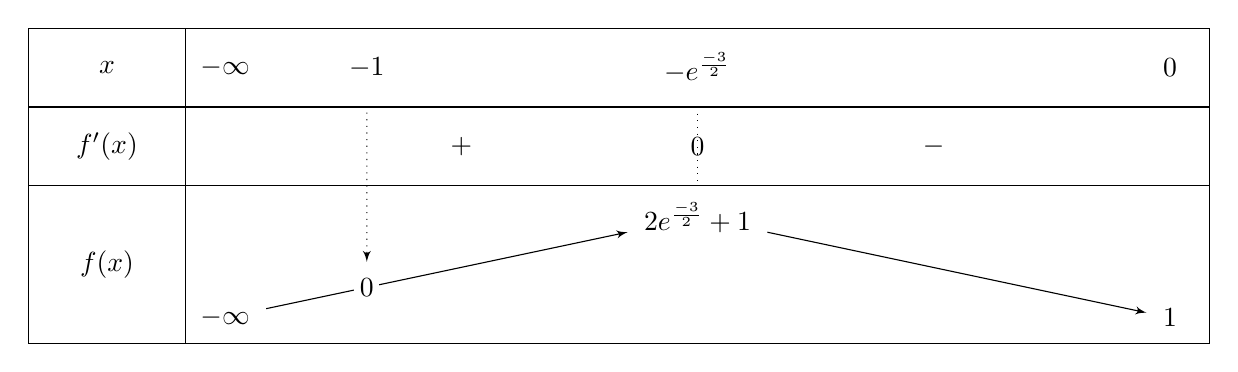
\begin{tikzpicture}
                            \tkzTabInit[espcl=6]
                            {$x$ / 1 , $f'(x)$ / 1, $f(x)$ / 2 }
                            {$-\infty$, $-e^{\frac{-3}{2}}$, $0$}
                            \tkzTabLine
                            {, +, z , -,}
                            \tkzTabVar
                            { -/$-\infty$ , +/$2e^{\frac{-3}{2}} + 1$, -/$1$}
                            \tkzTabVal[draw]{1}{2}{0.3}{$-1$}{$0$}
                        \end{tikzpicture}
                    \end{center}

\(
\begin{aligned}
g(-e^{\frac{-3}{2}}) &= 2(-e^{\frac{-3}{2}}) \ln(-(-e^{\frac{-3}{2}})) + (-e^{\frac{-3}{2}}) + 1 \\
&= -2e^{\frac{-3}{2}} \ln e^{\frac{-3}{2}} - e^{\frac{-3}{2}} + 1\\
&= -2e^{\frac{-3}{2}} \times \frac{-3}{2} - e^{\frac{-3}{2}} + 1 \\
&= 3e^{\frac{-3}{2}} - e^{\frac{-3}{2}} + 1 \\
&= 2e^{\frac{-3}{2}} + 1.
\end{aligned}
\)

          \begin{resultbox}
              \[
                  \mathbf{g(-e^{\frac{-3}{2}})=2e^{\frac{-3}{2}} + 1}
              \]
          \end{resultbox}        
        
          \item Calculons \( g(-1) \).\hfill \textbf{(0,75 pt)}
          
\(
\begin{aligned}
g(-1) &= 2(-1) \ln(-(-1)) + (-1) + 1 \\
&= -2 \ln(1) - 1 + 1\\
g(-1) &= -2 \times 0 - 1 + 1 \\
&= 0.
\end{aligned}
\)

          \begin{resultbox}
              \[
                  \mathbf{g(-1)=0}
              \]
          \end{resultbox} 

Le signe de \( g(x) \)

D'après le tableau de variation:

          \(
            \begin{cases}
              \forall x \in \left]-\infty;-1\right[, g(x)<0  \\
              \forall x \in \left]-1;0\right[, g(x)>0       
          \end{cases} 
          \)
\end{enumerate}

\subsection*{\underline{\textbf{Partie B}}:\textbf{ 7 pts}}

On considère la fonction \( f \) définie par :

\[
    f(x) =
    \begin{cases}
        x^2 \ln(-x) + x + 1 & \text{si } x < 0 \\
        x \ln(x)^2 + x + 1  & \text{si } x > 0 \\
        1                   & \text{si } x = 0
    \end{cases}
\]

On note \( (C_f) \) sa courbe représentative dans un repère orthonormé.

\begin{enumerate}
    \item Justifions que \( f \) est définie sur \( \mathbb{R} \).\hfill \textbf{(0,5 pt)}

		\[ \text{Posons }
    f(x) =
    \begin{cases}
        f_{1}(x)=x^2 \ln(-x) + x + 1 & \text{si } x < 0 \\
        f_{2}(x)=x \ln(x)^2 + x + 1  & \text{si } x > 0 \\
        f_{3}(x)=1                   & \text{si } x = 0
    \end{cases}
\]    
    
*\(f_{1}\) existe ssi \(-x > 0\)
    
    \(
    \begin{aligned}
    -x > 0 &\implies x < 0\\
    			 &\implies x \in]-\infty;0[
    \end{aligned}
    \)
    
    \underline{\(Df_{1} = ]-\infty;0[ \)}
    
*\(f_{2}\) existe ssi \(x > 0\)
    
    \(
    \begin{aligned}
    x > 0 &\implies x \in]-\infty;0[
    \end{aligned}
    \)
    
    \underline{\(Df_{2} = \in]-\infty;0[ \)}
    
    \underline{\(Df_{3} = \{0\} \)}
    
Donc 

\(
\begin{aligned}
Df&=Df_{1} \cup Df_{2} \cup Df_{3}\\
&=]-\infty;0[ \cup ]-\infty;0[\cup\{0\}\\
&=\mathbb{R}
\end{aligned}
\)

\begin{resultbox}
    \[
        \mathbf{Df=\mathbb{R}}
    \]
\end{resultbox} 

\item Étudions la continuité et la dérivabilité de \( f \) en 0. \hfill \textbf{(1,5 pt)}

\underline{\textbf{Continuité}}

\underline{En \( 0^- \), on a :} \( f(x) = x^2 \ln(-x) + x + 1. \)

\(
\begin{aligned}
     \lim\limits_{x \to 0^-}x^2 \ln(-x) + x + 1:
    \begin{cases}
        \lim\limits_{x \to 0^-}x^2 \ln(-x)=0 \\
       \lim\limits_{x \to 0^-} x + 1 =1
    \end{cases}\text{ Par somme}: \lim\limits_{x \to 0^-}x^2 \ln(-x) + x + 1 = 1
\end{aligned}
\)

Ainsi,
\begin{resultbox}
    \[
        \mathbf{\lim\limits_{x \to 0^-} f(x) = 1}
    \]
\end{resultbox} 

\underline{En \( 0^+ \), on a :} \( f(x) = x \ln(x)^2 + x + 1. \)

\(
\begin{aligned}
    \lim\limits_{x \to 0^+} x \ln(x)^2 + x + 1:
    \begin{cases}
        \lim\limits_{x \to 0^+} (x^{\frac{1}{2}} \ln(x))^2 = 0, \\
        \lim\limits_{x \to 0^+} x + 1 = 1.
    \end{cases}
    \text{ Par somme : } \lim\limits_{x \to 0^+} f(x) = 1.
\end{aligned}
\)

Ainsi,

\begin{resultbox}
    \[
        \mathbf{\lim\limits_{x \to 0^+} f(x) = 1}
    \]
\end{resultbox} 

\textbf{  Conclusion }

On sait que \( f(0) = 1 \). De plus :

\begin{resultbox}
    \[
        \mathbf{\lim\limits_{x \to 0^-} f(x) = \lim\limits_{x \to 0^+} f(x) = f(0) = 1.
        }
    \]
\end{resultbox} 

Par conséquent, la fonction \( f \) est \textbf{continue en \( x = 0 \)}.

\underline{\textbf{Dérivabilité}}

\underline{En \( 0^- \), on a :} \( f(x) = x^2 \ln(-x) + x + 1. \)

\( 
\begin{aligned}
    \lim\limits_{x \to 0^-}\frac{f(x)-f(0)}{x-0} &=\lim\limits_{x \to 0^-} \frac{x^2 \ln(-x) + x + 1-1}{x}\\
    &=\lim\limits_{x \to 0^-} \frac{x^2 \ln(-x) + x }{x}\\
    &=\lim\limits_{x \to 0^-} x \ln(-x) + 1\\
    &=1
\end{aligned} 
\)

\begin{resultbox}
    \[
        \mathbf{\lim\limits_{x \to 0^-}\frac{f(x)-f(0)}{x-0}=1
        }
    \]
\end{resultbox} 

\underline{En \( 0^+ \), on a :} \( f(x) = x \ln(x)^2 + x + 1. \)

\( 
\begin{aligned}
    \lim\limits_{x \to 0^+}\frac{f(x)-f(0)}{x-0} &=\lim\limits_{x \to 0^+} \frac{x \ln(x)^2 + x + 1-1}{x}\\
    &=\lim\limits_{x \to 0^+} \frac{x \ln(x)^2 + x }{x}\\
    &=\lim\limits_{x \to 0^+} \ln(x)^2+1\\
    &=1
\end{aligned} 
\)

\begin{resultbox}
    \[
        \mathbf{\lim\limits_{x \to 0^+}\frac{f(x)-f(0)}{x-0}=1
        }
    \]
\end{resultbox} 

\begin{resultbox}
    \[
        \mathbf{\lim\limits_{x \to 0^-}\frac{f(x)-f(0)}{x-0}=\lim\limits_{x \to 0^+}\frac{f(x)-f(0)}{x-0}=1
        }
    \]
\end{resultbox} 

Par conséquent, la fonction \( f \) est \textbf{dérivable en \( x = 0 \)}.

Interprétons graphiquement les résultats:

\( f \) est dérivable en 0 et admet une tangeant d'équation \( y=x \)

    \item Donnons le domaine de dérivabilité de \( f \) puis montrons que
          \(
              f'(x) =
              \begin{cases}
                  g(x)          & \text{si } x < 0 \\
                  (1 + \ln x)^2 & \text{si } x > 0
              \end{cases}
          \)\hfill \textbf{(0,5$\times$3 pts)}

\textbf{\underline{Domaine de dérivabilité}}

\( f_{1}(x)=x^2 \ln(-x) + x + 1 \) est dérivable si \( x < 0 \) ainsi \( Df_{1}' = ]-\infty;0[\) 

\( f_{2}(x)=x \ln(x)^2 + x + 1  \) est dérivable si \(  x > 0 \) ainsi \( Df_{2}' = ]0;+\infty[\) 

D'après ce qui précède, \(f\) est dérivable en 0 donc f est bien dérivable sur \(\mathbb{R}\).

ainsi 

\( 
\begin{aligned}
    Df'&=Df_{1}' \cup Df_{2}' \cup Df_{3}\\
        &=]-\infty;0[ \cup ]0;+\infty[ \cup  \{0\}\\
        &=\mathbb{R}
\end{aligned} 
\)

\begin{resultbox}
    \[
        \mathbf{Df'=\mathbb{R} }
    \]
\end{resultbox} 

\(
\begin{aligned}
        f'(x) &=
    \begin{cases}
        [x^2 \ln(-x) + x + 1]' & \text{si } x < 0 \\
        [x \ln(x)^2 + x + 1]'  & \text{si } x > 0 \\
    \end{cases}\\
    &=
    \begin{cases}
        (x^2 \ln(-x))' + (x + 1)' & \text{si } x < 0 \\
        (x \ln(x)^2)' + (x + 1)'  & \text{si } x > 0 \\
    \end{cases}\\
    &=
    \begin{cases}
        2x \ln(-x) + x^2\times\frac{1}{x} + 1 & \text{si } x < 0 \\
        \ln(x)^2+2x\times\frac{1}{x}\times\ln(x) + 1  & \text{si } x > 0 \\
    \end{cases}\\
    &=
    \begin{cases}
        2x \ln(-x) + x + 1 & \text{si } x < 0 \\
        \ln(x)^2+2\ln(x) + 1  & \text{si } x > 0 \\
    \end{cases}\\
    &=
    \begin{cases}
        g(x) & \text{si } x < 0 \\
        (\ln(x)+1)^{2}  & \text{si } x > 0 \\
    \end{cases}\textbf{ cqfd}
\end{aligned}
\)

\item Calculons les limites de \( f \) aux bornes de son domaine de définition.\hfill \textbf{(0,5 pt)}

\underline{En \( -\infty \), on a :} \( f(x) = x^2 \ln(-x) + x + 1 \)

\(
\begin{aligned}
    \lim\limits_{x\to -\infty} f(x) &= \lim\limits_{x\to -\infty} x^2 \ln(-x) + x + 1\\
    &= \lim\limits_{x\to -\infty} x^{2} \left[\ln(-x) + \frac{x + 1}{x}\right]\\
    &= +\infty \left[+\infty+1 \right]\\
    &=+\infty
\end{aligned}
\)

\begin{resultbox}
    \[
        \mathbf{\lim\limits_{x\to -\infty} f(x) = +\infty }
    \]
\end{resultbox} 

\underline{En \( +\infty \), on a :} \( f(x) = x \ln(x)^2 + x + 1. \)

\(
\begin{aligned}
    \lim\limits_{x\to +\infty} f(x) &= \lim\limits_{x\to +\infty}  x \ln(x)^2 + x + 1\\
    &=+\infty
\end{aligned}
\)

\begin{resultbox}
    \[
        \mathbf{\lim\limits_{x\to +\infty} f(x) = +\infty }
    \]
\end{resultbox} 

\item Étudions les branches infinies de \( (C_f) \).\hfill \textbf{(0,5 pt)}

Comme \( \lim\limits_{x\to -\infty} f(x) = +\infty  \) calculons \( \lim\limits_{x\to -\infty} \frac{f(x)}{x}   \)

En effet 

\( 
\begin{aligned}
    \lim\limits_{x\to -\infty} \frac{f(x)}{x} &= \lim\limits_{x\to -\infty} \frac{x^2 \ln(-x) + x + 1}{x}\\
    &=\lim\limits_{x\to -\infty} x\ln(-x) + \frac{x + 1}{x}\\
    &=-\infty+1\\
    &=-\infty
\end{aligned} 
\)

Donc \( \lim\limits_{x\to -\infty} \frac{f(x)}{x} =+\infty   \)

\textcolor{red}{Donc \(Cf\) admet une branche parabolique de direction \((Oy)\) au voisinage de \(-\infty\)}

Comme \( \lim\limits_{x\to +\infty} f(x) = +\infty  \) calculons \( \lim\limits_{x\to +\infty} \frac{f(x)}{x}   \)

En effet 

\( 
\begin{aligned}
    \lim\limits_{x\to +\infty} \frac{f(x)}{x} &= \lim\limits_{x\to +\infty} \frac{x \ln(x)^2 + x + 1}{x}\\
    &=\lim\limits_{x\to +\infty} \ln(x)^2 + \frac{x + 1}{x}\\
    &=+\infty+1\\
    &=+\infty
\end{aligned} 
\)

Donc \( \lim\limits_{x\to +\infty} \frac{f(x)}{x} =-\infty   \)

\textcolor{red}{Donc \((Cf)\) admet une branche parabolique de direction \((Oy)\) au voisinage de \(+\infty\)}
    \item Dressons le tableau de variations de \( f \).\hfill \textbf{(1 pt)}

Le signe de \( f \).  on a : \(
              f'(x) =
              \begin{cases}
                  g(x)          & \text{si } x < 0 \\
                  (1 + \ln x)^2 & \text{si } x > 0
              \end{cases}
          \)\hfill \textbf{(0,5$\times$3 pts)}

          \(
            \begin{cases}
              \forall x \in \left]-\infty;-1\right[, g(x)<0 \text{ donc \(f\) est y décroissante}\\
              \forall x \in \left]-1;0\right[, g(x)>0 \text{ donc \(f\) y est croissante}\\
              \forall x \in \left]0;-\infty\right[, f(x)>0
          \end{cases} 
          \)
    
        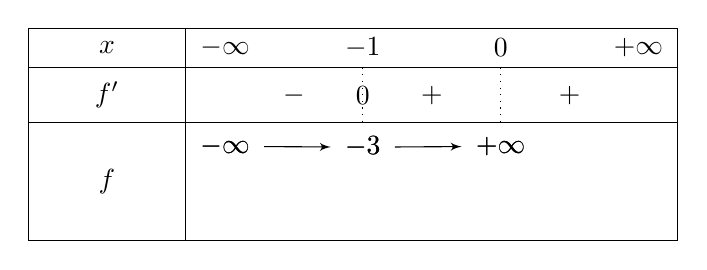
\begin{tikzpicture}[node style/.style={fill opacity=0,text opacity=1}]
        \tkzTabInit[espcl=1.75]{$x$/.5,$f'$/.7,$f$/1.5}{$-\infty$,$-1$,$0$,$+\infty$}
        \tkzTabLine{,-,z,+,t,+,}
        \tkzTabVar{+/$-\infty$,+/$-3$,+/$+\infty$}
    		\end{tikzpicture}
    		

    %\item Montrer que dans \( ]-\infty; -1[ \), l’équation \( f(x) = 1 \)

         % admet une unique solution \( \alpha \) puis vérifier que \(-1,8 < \alpha < -1,7\).\hfill \textbf{(0,75 pt)}
    %\item Construire \( (C_f) \) (unité 2 cm) (on précisera la tangente au point d’abscisse \( e^{-1} \) et on placera le point d’abscisse 1).\hfill \textbf{(0,75 pt)}
\end{enumerate}

\end{document}